\iffalse
\let\negmedspace\undefined
\let\negthickspace\undefined
\documentclass[journal,12pt,twocolumn]{IEEEtran}
\usepackage{cite}
\usepackage{amsmath,amssymb,amsfonts}
\usepackage{graphicx}
\usepackage{textcomp}
\usepackage{xcolor}
\usepackage{txfonts}
\usepackage{listings}
\usepackage{enumitem}
\usepackage{mathtools}
\usepackage{gensymb}
\usepackage{comment}
\usepackage[breaklinks=true]{hyperref}
\usepackage{tkz-euclide} 
\usepackage{listings}
\usepackage{gvv}                                        
\def\inputGnumericTable{}                                 
\usepackage[latin1]{inputenc}                                
\usepackage{color}                                            
\usepackage{array}                                            
\usepackage{longtable}                                       
\usepackage{calc}                                             
\usepackage{multirow}                                         
\usepackage{hhline}                                           
\usepackage{ifthen}                                           
\usepackage{lscape}
\usepackage[export]{adjustbox}

\newtheorem{theorem}{Theorem}[section]
\newtheorem{problem}{Problem}
\newtheorem{proposition}{Proposition}[section]
\newtheorem{lemma}{Lemma}[section]
\newtheorem{corollary}[theorem]{Corollary}
\newtheorem{example}{Example}[section]
\newtheorem{definition}[problem]{Definition}
\newcommand{\BEQA}{\begin{eqnarray}}
\newcommand{\EEQA}{\end{eqnarray}}
\newcommand{\define}{\stackrel{\triangle}{=}}
\newtheorem{rem}{Remark}

\begin{document}
\parindent 0px
\bibliographystyle{IEEEtran}
\fi
\vspace{3cm}

\title{}
\author{EE23BTECH11042 -  Khusinadha Naik$^{*}$
}
\maketitle
\newpage
\bigskip

% \renewcommand{\thefigure}{\theenumi}
% \renewcommand{\thetable}{\theenumi}


\noindent \textbf{26.} \hspace{2pt}A causal, discrete time system is described by the difference equation $y[n] = 0.5 y[n-1] + x[n]$, for all $n$, where $y[n]$ denotes the output sequence and $x[n]$ denotes the input sequence. Which of the following statements is/are TRUE?
\begin{flushright}
\hfill(GATE 2023 BM)
\end{flushright}
\begin{enumerate}[label = (\alph*)]
	\item The system has an impulse response described by $0.5^{n} u[-n]$ where $u[n]$ is the  
unit step sequence. 	\label{option:GATE.2023.BM.26.1}	
	\item The system is stable in the bounded input, bounded output sense.		\label{option:GATE.2023.BM.26.2}
	\item The system has an infinite number of non-zero samples in its impulse response	\label{option:GATE.2023.BM.26.3}
	\item The system has a finite number of non-zero samples in its impulse response.	\label{option:GATE.2023.BM.26.4}
\end{enumerate}

\noindent \textbf{Ans.}\\
\begin{table}[h]
\centering
\begin{tabular}{|c|c|c|}
        \hline
        \textbf{Parameter} & \textbf{Value} & \textbf{Description} \\
        \hline
        $x[n]$ & ? & Input Sequence \\
        \hline
        $y[n]$ & ? & Output Sequence \\
        \hline
        
\end{tabular}
\caption{Input parameters table}
\label{tab:GATE.2023.BM.26.1}





\end{table}
\begin{align}
y[n] = 0.5y[n-1] + x[n] 
\end{align}

Taking $Z$-Transform 
\begin{align}
Y\brak{Z} &= 0.5Z^{-1}Y\brak{Z} + X\brak{Z} \\
\implies \frac{Y\brak{Z}}{X\brak{Z}} &= \frac{1}{1 - 0.5z^{-1}} = H\brak{Z} 
\end{align}
If $x[n]$ is impulse input 
\begin{align}
& X\brak{Z} = 1 \\
\implies &Y\brak{Z} = H\brak{Z} = \frac{1}{1 - 0.5z^{-1}} 
\end{align}
Taking inverse $Z$-Transform
\begin{align}
y[n] = h[n] = 0.5^{n}u[n]
\end{align}
Hence \ref{option:GATE.2023.BM.26.1} is wrong,\\

$y[n]$ is a non-zero infinite G.P. hence \ref{option:GATE.2023.BM.26.3} holds true and \ref{option:GATE.2023.BM.26.4} is false

\pagebreak
Plotting $y[n]$ vs $n$
\begin{figure}[h]
    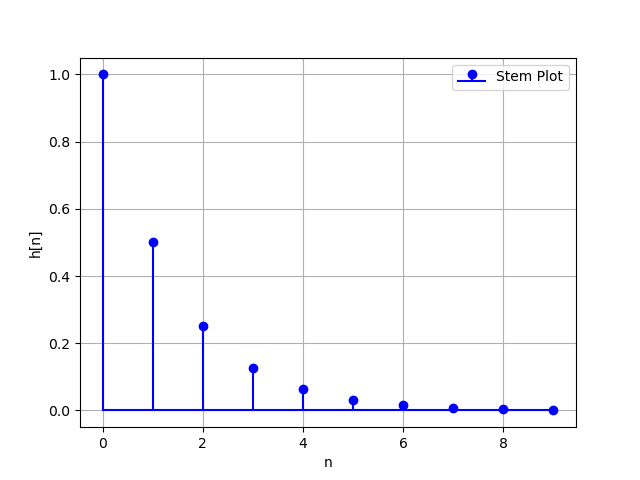
\includegraphics[width=0.5\textwidth]{gate-signal/2023/BM/26/figs/fig1.png}
    \caption{Plot of $y[n]$ vs $n$}
    \label{fig:GATE.2023.BM.26.1}
\end{figure}


To check BIBO stability we'll check absolute convergence of values for $h[n]$
\begin{align}
&= \sum^{+\infty}_{n = -\infty}\abs{\:h[n]\:} \\
&= \sum^{+\infty}_{n = -\infty}\abs{\:0.5^nu[n]\:}
\end{align}
It's a infinite G.P. with a = 1 , r = 0.5
\begin{align}
\sum^{+\infty}_{n = -\infty}\abs{\:0.5^nu[n]\:} &= \frac{a}{1 -r} \\
&= \frac{1}{1 - 0.5} = 2
\end{align}
As it is a finite value it is BIBO stable so \ref{option:GATE.2023.BM.26.2} holds true.









%\end{document}
